% 2016_zhejiang_science_q17_fig1: triangular frustum ABC-DEF, AC dashed (same layout as liberal q18)
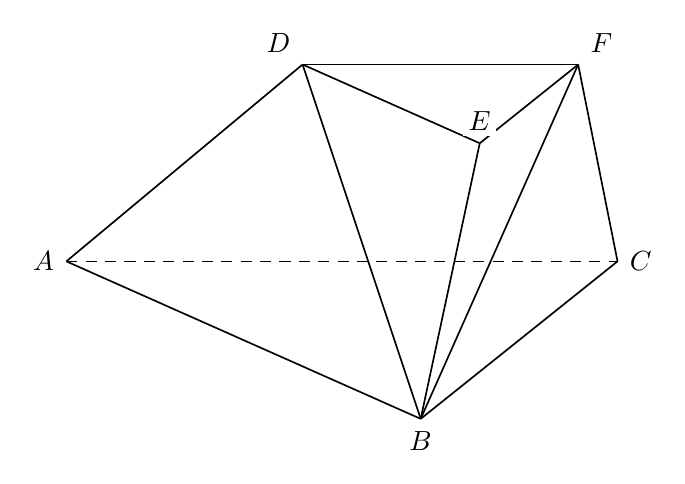
\begin{tikzpicture}[x=1cm,y=1cm,font=\normalsize]
\tikzset{solid edge/.style={solid,line width=.6pt},dashed edge/.style={dashed,dash pattern=on 4pt off 3pt,line width=.6pt},ptlabel/.style={fill=white,draw=none,inner sep=2pt,font=\normalsize}}
\coordinate (A) at (0,2.5);
\coordinate (C) at (7.0,2.5);
\coordinate (B) at (4.5,0.5);
\coordinate (D) at (3.0,5.0);
\coordinate (F) at (6.5,5.0);
\coordinate (E) at (5.2500000000,4.0000000000);
\draw[solid edge] (A)--(D);
\draw[solid edge] (D)--(F);
\draw[solid edge] (F)--(C);
\draw[solid edge] (A)--(B);
\draw[solid edge] (B)--(C);
\draw[solid edge] (D)--(B);
\draw[solid edge] (B)--(E);
\draw[solid edge] (E)--(F);
\draw[solid edge] (D)--(E);
\draw[solid edge] (B)--(F);
\draw[dashed edge] (A)--(C);
\node[ptlabel,anchor=east] at ([xshift=-.8mm]A) {$A$};
\node[ptlabel,anchor=west] at ([xshift=.8mm]C) {$C$};
\node[ptlabel,anchor=north] at ([yshift=-.8mm]B) {$B$};
\node[ptlabel,anchor=south east] at ([xshift=-.8mm,yshift=.8mm]D) {$D$};
\node[ptlabel,anchor=south west] at ([xshift=.8mm,yshift=.8mm]F) {$F$};
\node[ptlabel,anchor=south] at ([yshift=.8mm]E) {$E$};
\end{tikzpicture}
